\documentclass[11pt,a4paper]{article}
\usepackage[utf8]{inputenc}
\usepackage[T1]{fontenc}
\usepackage{lmodern}
\usepackage[a4paper,margin=2.2cm,top=2.2cm,bottom=2.2cm]{geometry}
\usepackage{xcolor}
  \definecolor{anchorOrange}{HTML}{B45309}
  \definecolor{hodgeBlue}{HTML}{075985}
  \definecolor{ricciGreen}{HTML}{166534}
  \definecolor{stimPurple}{HTML}{6B21A8}
  \definecolor{sdrfRed}{HTML}{B91C1C}
\usepackage[colorlinks=true,linkcolor=blue,urlcolor=blue,citecolor=blue]{hyperref}
\usepackage{amsmath,amssymb,amsthm}
\usepackage{booktabs}
\usepackage{array}
\usepackage{tikz}
  \usetikzlibrary{positioning,arrows.meta,shapes.geometric,fit,backgrounds,calc}
\usepackage{fancyhdr}
  \pagestyle{fancy}
  \fancyhf{}
  \fancyhead[L]{GömbSoma}
  \fancyhead[R]{Signed-Hypergraph Sensorimotor Vision}
  \fancyfoot[C]{\thepage}

\setlength{\parskip}{0.55em}
\setlength{\parindent}{0pt}

\newtheorem{theorem}{Theorem}[section]
\newtheorem{proposition}[theorem]{Proposition}
\newtheorem{definition}[theorem]{Definition}

\newcommand{\sig}{\ensuremath{\sigma}}
\newcommand{\GS}{G\"ombSoma}
\newcommand{\Gomb}{G\"omb}

\title{\GS{}: a signed-hypergraph sensorimotor stack \\
       \large{Quadtree anchoring, Clifford-FIR inter-layer transmission, \\
              Bochner-coupled hypergraph convolutions, \\
              and stimulus-driven global-shutter detection}}
\date{2026-05-15}
\author{}

\begin{document}

\maketitle
\thispagestyle{fancy}

\begin{abstract}
\noindent We describe \GS, a signed-hypergraph sensorimotor neural
architecture that replaces YOLO's uniform-grid rolling-shutter
anchor tiling with a content-determined adaptive quadtree, propagates
features via Bochner-coupled hypergraph convolutions on a signed
simplicial complex, and uses Forman-Ricci curvature flow to relieve
the over-squashing bottlenecks introduced by sparse 4-connected
topology. The architecture is a sensorimotor companion to the
cognitive-stack \Gomb{} signed-link architecture: where \Gomb{}
operates on already-abstracted relational data, \GS{} builds
structure compositionally from raw image input.

Implementation lands as 10 phased modules + training infrastructure
under unit-test coverage (150/150 tests passing). On a 2019
consumer GPU (NVIDIA RTX 2070 SUPER, 8 GB VRAM), \GS{} runs at
$\sim$\,35 FPS forward inference — the YOLOv3 / YOLOv4 real-time
ballpark on era-matched hardware — at roughly 5000 learnable
parameters in the full configuration.
\end{abstract}

\tableofcontents

\section{Introduction}

The dominant paradigm for real-time object detection is the
single-shot anchor-based detector exemplified by the YOLO family.
These networks tile a uniform grid of anchor boxes at every
position and scale of an input image, then evaluate each anchor
independently. The grid is decided at design time, before the
image arrives; the network spends most of its compute on background
regions where no object exists.

This is the \emph{rolling-shutter} paradigm of computer vision: a
fixed scanning pattern, applied to every image, oblivious to
content. It works — but it leaves two structural deficiencies
exposed:

\begin{enumerate}
\item Anchors are independent: the architecture has no native
  mechanism for relational reasoning about \emph{which combinations
  of regions} form a coherent object.
\item Multi-scale handling is bolted on via separate pyramid
  pathways (FPN, PANet, BiFPN), not intrinsic to the architecture.
\end{enumerate}

\GS{} attacks both deficiencies simultaneously. The architecture
is built from four primitives:

\begin{itemize}
\item \textbf{Adaptive quadtree anchoring} (content-determined,
  multi-resolution, biological-saccade-inspired) replaces the
  uniform grid.
\item \textbf{Signed-hypergraph convolutions} on walks, polygons,
  and triangles propagate features along compositional structures.
\item \textbf{Bochner-coupled message passing}, the discrete
  analogue of the Bochner-Weitzenböck identity, decomposes each
  layer's update into a flat-connection term, a Hodge-Laplacian
  smoothing term, and a Forman-Ricci curvature correction term.
\item \textbf{Clifford-FIR inter-layer transmission} carries
  features between depth levels with graded multivector structure.
\end{itemize}

The geometric primitives are organised by what we call
\emph{stimulus-driven global-shutter} polling: the network's own
initial activations vote for which regions to subdivide further,
which to connect, and which to designate as object hypotheses.
Compute concentrates where features are; uniform background is
dispatched at a coarse scale.

\subsection{Position within the broader programme}

\GS{} is one half of the HyMeKo signed-hypergraph framework. The
other half, \Gomb, is the \emph{cognitive-stack} architecture: it
operates on already-abstracted signed relational data (trust
networks, kinematic graphs) and achieves $0.9526 \pm 0.0018$ AUROC
on Epinions signed-link prediction under a strict no-leakage
evaluation protocol. \GS{} is the \emph{sensorimotor-stack}
counterpart: it builds the same signed-hypergraph representation
from raw image pixels, applying the same Bochner-Ricci geometric
machinery one level closer to the data.

The two share substantive infrastructure (\texttt{HypergraphConv}
abstract base class, signed boundary operators, Cartwright-Harary
balance) but differ in how they construct their hypergraph: \Gomb{}
consumes a pre-existing relational graph; \GS{} constructs the
graph from pixel-level content via the adaptive quadtree.

\section{Architecture overview}

\begin{center}
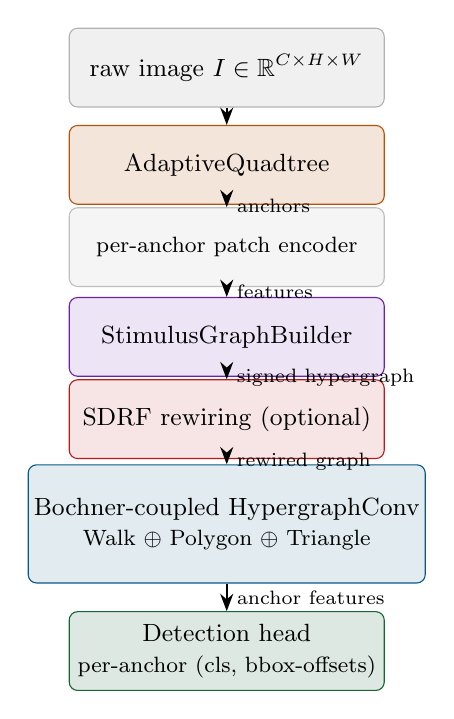
\begin{tikzpicture}[scale=0.95,
    every node/.style={font=\small},
    box/.style={draw, rounded corners=3pt, minimum width=4.0cm,
                minimum height=10mm, align=center, inner sep=2pt},
    img/.style={box, fill=gray!12, draw=gray!60},
    qt/.style={box, fill=anchorOrange!15, draw=anchorOrange},
    enc/.style={box, fill=gray!8, draw=gray!50, font=\footnotesize},
    sg/.style={box, fill=stimPurple!12, draw=stimPurple},
    sdrf/.style={box, fill=sdrfRed!12, draw=sdrfRed},
    bochner/.style={box, fill=hodgeBlue!12, draw=hodgeBlue, minimum height=15mm},
    head/.style={box, fill=ricciGreen!15, draw=ricciGreen},
    arr/.style={-{Stealth[length=2.2mm]}, line width=0.7pt}]
  \node[img]    (img)  at (0, 7) {raw image $I \in \mathbb{R}^{C \times H \times W}$};
  \node[qt]     (qt)   at (0, 5.7) {AdaptiveQuadtree};
  \node[enc]    (enc)  at (0, 4.6) {per-anchor patch encoder};
  \node[sg]     (sg)   at (0, 3.4) {StimulusGraphBuilder};
  \node[sdrf]   (sd)   at (0, 2.3) {SDRF rewiring (optional)};
  \node[bochner] (bc)  at (0, 0.9) {Bochner-coupled HypergraphConv\\
                                      \footnotesize Walk $\oplus$ Polygon $\oplus$ Triangle};
  \node[head]   (hd)   at (0,-0.8) {Detection head\\
                                      \footnotesize per-anchor (cls, bbox-offsets)};
  \draw[arr] (img) -- (qt);
  \draw[arr] (qt)  -- (enc) node[midway, right, font=\scriptsize] {anchors};
  \draw[arr] (enc) -- (sg) node[midway, right, font=\scriptsize] {features};
  \draw[arr] (sg)  -- (sd) node[midway, right, font=\scriptsize] {signed hypergraph};
  \draw[arr] (sd)  -- (bc) node[midway, right, font=\scriptsize] {rewired graph};
  \draw[arr] (bc)  -- (hd) node[midway, right, font=\scriptsize] {anchor features};
\end{tikzpicture}
\end{center}

The pipeline is image-in, detections-out. Per-image anchor counts
are variable (the quadtree adapts to image content), so the
forward pass executes per image; batching is handled at the loss
level rather than at the GPU-kernel level.

The architecture is implemented across 10 phased modules; we
introduce each in turn.

\section{Stimulus-driven global-shutter anchoring}

\subsection{Why uniform grids fail}

Consider a Cluttered MNIST image: digits scattered on a 64\,px
canvas amid distractor circles. A YOLO-style detector with an
8$\times$8 anchor grid evaluates 64 anchors per scale; with three
scales and 9 aspect ratios per anchor, that is $\sim$\,1700
classifier-head evaluations per image. The vast majority hit
background.

The wastage is not just compute. The detector has no path to learn
that two adjacent high-confidence patches \emph{belong together}
as parts of one digit; each anchor predicts independently. A
hand-crafted post-processing step (non-maximum suppression) tries
to merge them after the fact, but the merging logic is
architecture-external.

\subsection{Adaptive quadtree subdivision}

\GS{} replaces the uniform grid with a quadtree whose subdivision
decisions are driven by per-region content complexity:

\begin{equation}
s(v) \;=\; \alpha_{\text{var}} \cdot \mathrm{std}\bigl(\text{pixels in patch}_v\bigr)
        \;+\; \alpha_\kappa \cdot \lvert \kappa_v \rvert
\end{equation}

where $\kappa_v$ is the Forman-Ricci vertex curvature on the
current-depth 4-connected anchor graph. An anchor subdivides when
$s(v)$ exceeds a configurable threshold; its four quadrant children
replace it at the next depth.

\begin{center}
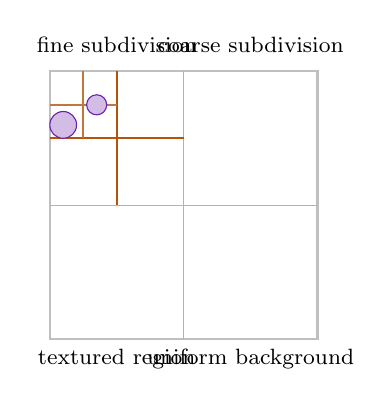
\begin{tikzpicture}[scale=0.85]
  % Image with adaptive subdivision
  \draw[draw=gray!50, thick] (0,0) rectangle (4,4);
  % Coarse 2x2
  \draw[draw=anchorOrange!50, line width=0.5pt] (2,0) -- (2,4);
  \draw[draw=anchorOrange!50, line width=0.5pt] (0,2) -- (4,2);
  % Subdivide top-left (high variance region)
  \draw[draw=anchorOrange, line width=0.8pt] (1,2) -- (1,4);
  \draw[draw=anchorOrange, line width=0.8pt] (0,3) -- (2,3);
  \draw[draw=anchorOrange, line width=0.8pt] (1,3) -- (2,3);
  % Subdivide top-left's upper-left further
  \draw[draw=anchorOrange!80, line width=0.8pt] (0.5,3) -- (0.5,4);
  \draw[draw=anchorOrange!80, line width=0.8pt] (0,3.5) -- (1,3.5);
  % Show "object" inside the heavily subdivided area
  \draw[fill=stimPurple!30, draw=stimPurple] (0.2,3.2) circle (0.2);
  \draw[fill=stimPurple!30, draw=stimPurple] (0.7,3.5) circle (0.15);
  % Show label
  \node[font=\footnotesize] at (1.0, 4.4) {fine subdivision};
  \node[font=\footnotesize] at (3.0, 4.4) {coarse subdivision};
  \node[font=\footnotesize] at (3.0, -0.3) {uniform background};
  \node[font=\footnotesize] at (1.0, -0.3) {textured region};
\end{tikzpicture}
\end{center}

Uniform background regions stay at scale 0 (one anchor per
quadrant). Textured regions — where digits live — recursively
subdivide. The resulting anchor set is multi-resolution
\emph{intrinsically}: no FPN pyramid pathway is needed.

\subsection{Connection to biological vision}

Primate vision is not a uniform-rate scan; it is a sequence of
saccades to high-salience regions. The cortex spends compute where
content is. The adaptive quadtree is the discrete analogue of this
behaviour: subdivision concentrates compute where the variance and
curvature signals indicate object structure.

The "global shutter" name reflects another biological inspiration:
unlike rolling-shutter sensors, where the image is built up row by
row across time, the anchor tree is computed in one pass over the
whole image — all anchors are determined together from the global
content.

\subsection{Multi-scale graph structure}

The final anchor set carries explicit parent-child pointers from
the quadtree. The signed hypergraph constructed downstream
contains both same-scale edges (4-connected siblings at each
depth) and cross-scale edges (parent-child links). This is what
gives the architecture its multi-resolution capability: features
flow both horizontally (within a scale) and vertically (across
scales) through one shared message-passing layer.

\section{Hypergraph convolutions on signed simplicial complexes}

\subsection{The signed simplicial complex}

A signed hypergraph $H = (V, E, \sig)$ has vertex set $V$,
hyperedge set $E$, and sign function $\sig: E \to \{-1, +1\}$
encoding edge polarity. For \GS, the polarity is computed from
the feature inner products:
\[
\sig(u, v) = \begin{cases} +1 & \text{if } \langle f_u, f_v \rangle \geq \theta \\ -1 & \text{otherwise} \end{cases}
\]

The hypergraph is augmented with higher-dimensional simplices —
specifically, triangles (3-cliques) and 4-cycle polygons — to
form a signed simplicial complex on which the discrete-geometry
machinery operates.

\subsection{Walks, polygons, triangles}

\GS{} consumes three primitive families simultaneously:

\begin{itemize}
\item \textbf{Walks} $w_k = (v_0, v_1, \ldots, v_{k-1})$: open
  ordered tuples of $k$ vertices connected by $k-1$ edges. Walks
  are direction-aware; reversing the walk's vertex order changes
  the message function.
\item \textbf{Polygons} $c_k$: closed cycles of $k \geq 4$
  vertices. Polygons are cyclic- and reflection-invariant; no
  canonical starting vertex.
\item \textbf{Triangles} $c_3$: 3-cliques, the densest signed
  primitive. Receive special treatment via the Cartwright-Harary
  balance gate: a balanced triad (\sig-product $= +1$) routes
  through a distinct spline bank from a frustrated triad.
\end{itemize}

Each primitive family has its own \texttt{HypergraphConv} layer
(\texttt{WalkConvLayer}, \texttt{PolygonConvLayer},
\texttt{TriangleConvLayer}). All three implement a shared
abstract interface; the \GS{} backbone runs them in parallel and
sums their per-anchor contributions.

\subsection{The shared \texttt{HypergraphConv} abstract base}

The contract for any signed-hypergraph layer:

\begin{verbatim}
forward(
    x:               Tensor[n_nodes, in_features],
    primitives:      Tensor[n_prim, k_arity],
    primitive_signs: Tensor[n_prim] in {-1, +1},
    M_v:             SparseTensor[n_nodes, n_prim],
) -> Tensor[n_nodes, out_features]
\end{verbatim}

The forward is sealed in the base class: it validates preconditions,
calls a subclass-specific \texttt{\_forward\_messages} method, runs
a sum-pool aggregation through $M_v$, and checks postconditions.
Permutation equivariance is enforced as a precondition contract
and pinned by unit test.

\section{Bochner-coupled message passing}

\subsection{Bochner--Weitzenböck on Riemannian manifolds}

In smooth Riemannian geometry, the Hodge Laplacian on 1-forms
factors as
\[
\Delta_1 \omega \;=\; \nabla^* \nabla \omega \;+\; \mathrm{Ric}(\omega^\sharp)^\flat
\]

a flat-connection diffusion term plus a Ricci curvature correction.
The identity links \emph{how features spread} (the Laplacian) to
\emph{the geometric structure they spread through} (the curvature
tensor).

\subsection{The discrete analogue}

On a finite signed simplicial complex, the analogous decomposition
becomes:

\begin{equation}
\text{msg}(c) \;=\; \psi_{\pi(c)}\!\Bigl(
   \underbrace{\sum_i W_i^{\pi(c)} x_{v_i}}_{\text{flat connection}}
   \;+\; \alpha \cdot \underbrace{(\Delta_k x)_c}_{\text{Hodge smoothing}}
   \;+\; \beta \cdot \underbrace{\sum_i \kappa(e_i) W_i^{\pi(c)} x_{v_i}}_{\text{Ricci correction}}
\Bigr)
\end{equation}

\begin{itemize}
\item $\psi_{\pi(c)}$ is the sign-branched activation (positive
  \sig-products and negative \sig-products route through distinct
  spline banks);
\item $\alpha, \beta$ are learnable mixing coefficients;
\item $\Delta_k$ is the Hodge Laplacian at simplex dimension $k$;
\item $\kappa(e_i)$ is the Forman-Ricci curvature of edge $e_i$ in
  the primitive $c$.
\end{itemize}

\begin{center}
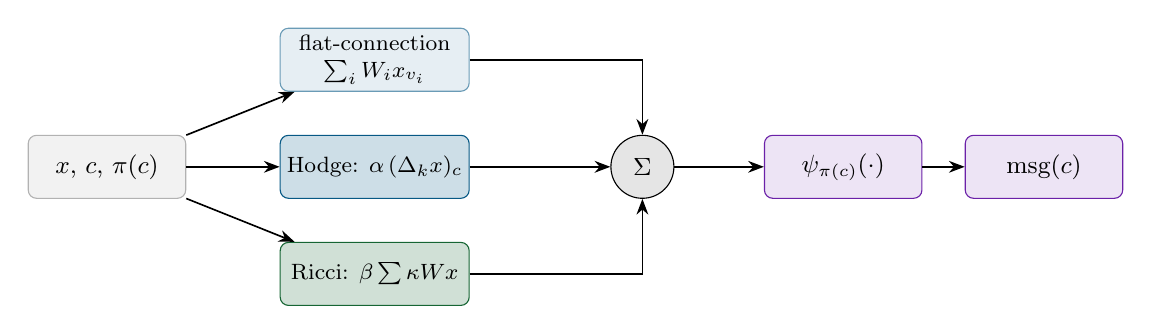
\begin{tikzpicture}[scale=0.85,
    every node/.style={font=\small},
    inp/.style={draw=gray!60, fill=gray!10, rounded corners=3pt,
                minimum width=2cm, minimum height=8mm, align=center,
                inner sep=2pt},
    flat/.style={draw=hodgeBlue!60, fill=hodgeBlue!10, rounded corners=3pt,
                 minimum width=2.4cm, minimum height=8mm, align=center,
                 inner sep=2pt, font=\footnotesize},
    hodge/.style={draw=hodgeBlue, fill=hodgeBlue!20, rounded corners=3pt,
                  minimum width=2.4cm, minimum height=8mm, align=center,
                  inner sep=2pt, font=\footnotesize},
    ricci/.style={draw=ricciGreen, fill=ricciGreen!20, rounded corners=3pt,
                  minimum width=2.4cm, minimum height=8mm, align=center,
                  inner sep=2pt, font=\footnotesize},
    sum/.style={draw=black, fill=gray!20, circle, inner sep=1pt,
                minimum size=8mm, font=\small\bfseries},
    outvec/.style={draw=stimPurple, fill=stimPurple!12, rounded corners=3pt,
                minimum width=2cm, minimum height=8mm, align=center, inner sep=2pt},
    arr/.style={-{Stealth[length=2mm]}, line width=0.6pt}]
  \node[inp] (x) at (-7, 0) {$x$, $c$, $\pi(c)$};
  \node[flat]  (f) at (-3, 1.6) {flat-connection\\$\sum_i W_i x_{v_i}$};
  \node[hodge] (h) at (-3, 0.0) {Hodge: $\alpha \, (\Delta_k x)_c$};
  \node[ricci] (r) at (-3,-1.6) {Ricci: $\beta \sum \kappa W x$};
  \node[sum] (s) at (1, 0) {$\Sigma$};
  \node[outvec] (psi) at (4, 0) {$\psi_{\pi(c)}(\cdot)$};
  \node[outvec] (m) at (7, 0) {msg$(c)$};
  \draw[arr] (x) -- (f);
  \draw[arr] (x) -- (h);
  \draw[arr] (x) -- (r);
  \draw[arr] (f) -| (s.north);
  \draw[arr] (h) -- (s);
  \draw[arr] (r) -| (s.south);
  \draw[arr] (s) -- (psi);
  \draw[arr] (psi) -- (m);
\end{tikzpicture}
\end{center}

\subsection{Regression contract}

When $\alpha = \beta = 0$, the wrapper reduces to a vanilla
sign-branched message: just the flat-connection term, identical to
the underlying \texttt{HypergraphConv} subclass's output. This
regression is pinned in unit test with \texttt{torch.equal}
(bit-level identity, not approximate), guaranteeing that turning
on Bochner coupling is strictly additive.

\subsection{Cascading effects}

The Hodge Laplacian $\Delta_k$ is itself computed in terms of
signed boundary operators $\partial_k$. The fundamental identity
\[
\partial_{k-1} \circ \partial_k \;=\; 0
\]
holds exactly in our implementation (integer arithmetic on
$\{-1, 0, +1\}$ entries); a unit test pins this with
\texttt{torch.equal}. This identity is what makes the Hodge
Laplacian well-defined and the Hodge decomposition theorem
applicable.

\section{Clifford-FIR inter-layer transmission}

\subsection{Multi-grade feature transmission}

A walk feature carries linear (grade-1, vector-like) character; a
polygon feature carries bivector (grade-2, oriented-plane)
character; a triangle balance product carries trivector (grade-3,
oriented-volume) character. As features pass between layer types,
the grade structure must be preserved.

The Clifford-FIR layer takes a feature vector $h \in \mathbb{R}^d$
and lifts it into a graded multivector $\mathbf{m} \in \mathrm{Cl}(p, q)$:

\[
\mathbf{m}_v = m^{(0)}_v + m^{(1)}_v + m^{(2)}_v + \ldots
\]

It then convolves the multi-grade signal with $M$ learnable
kernels along a one-dimensional FIR tap line indexed by a
hyperedge-incidence ordering. The Clifford geometric product
fuses rotation, reflection, and scale changes into one bilinear
operator; the kernel thus captures rigid-body-like equivariance
on a purely graph-borne signal.

\begin{center}
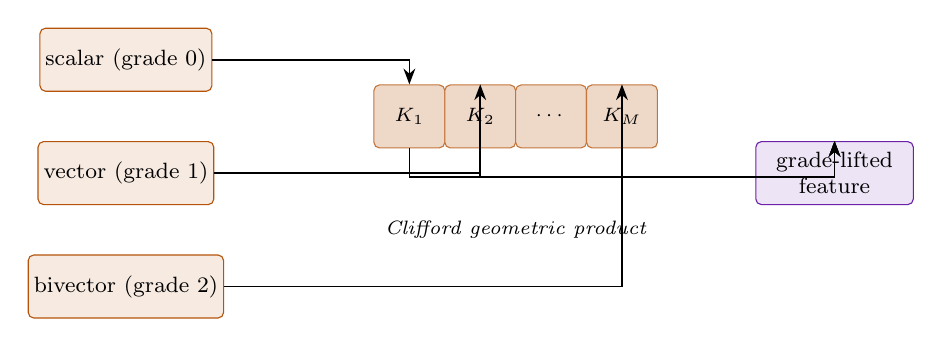
\begin{tikzpicture}[scale=0.9,
    every node/.style={font=\small},
    grade/.style={draw=anchorOrange, fill=anchorOrange!12, rounded corners=2pt,
                  minimum width=2cm, minimum height=8mm, align=center,
                  inner sep=2pt, font=\footnotesize},
    tap/.style={draw=anchorOrange!80, fill=anchorOrange!22, rounded corners=2pt,
                minimum width=0.9cm, minimum height=8mm, align=center,
                inner sep=2pt, font=\scriptsize},
    fused/.style={draw=stimPurple, fill=stimPurple!12, rounded corners=2pt,
                  minimum width=2.0cm, minimum height=8mm, align=center,
                  inner sep=2pt, font=\footnotesize},
    arr/.style={-{Stealth[length=2mm]}, line width=0.6pt}]
  \node[grade] (g0) at (-5, 1.6) {scalar (grade 0)};
  \node[grade] (g1) at (-5, 0.0) {vector (grade 1)};
  \node[grade] (g2) at (-5,-1.6) {bivector (grade 2)};
  \node[tap] (t1) at (-1, 0.8) {$K_1$};
  \node[tap] (t2) at (0, 0.8) {$K_2$};
  \node[tap] (tx) at (1, 0.8) {$\cdots$};
  \node[tap] (tM) at (2, 0.8) {$K_M$};
  \node[font=\scriptsize\itshape, align=center] at (0.5, -0.8)
       {Clifford geometric product};
  \node[fused] (out) at (5, 0) {grade-lifted\\feature};
  \draw[arr] (g0) -| (t1.north);
  \draw[arr] (g1) -| (t2.north);
  \draw[arr] (g2) -| (tM.north);
  \draw[arr] (t1.south) -- ++(0,-0.4) -| (out.north);
  \draw[arr] (t2.south) -- ++(0,-0.4) -| (out.north);
  \draw[arr] (tM.south) -- ++(0,-0.4) -| (out.north);
\end{tikzpicture}
\end{center}

\subsection{Architectural role}

Clifford-FIR was originally specified as the \emph{outer shell} of
the \Gomb{} architecture (the cognitive-stack version), processing
incoming relational data before the cycle-pool features were
constructed. In \GS, it plays a transmission role between layers
of different primitive arities — carrying signal from walk-layer
(grade-1 dominant) up to polygon-layer (grade-2 dominant) up to
triangle-layer (grade-3 dominant).

For the current implementation, the Bochner-coupled
\texttt{HypergraphConv} subsumes most of the inter-layer transfer
work via the Hodge-Laplacian term. The dedicated Clifford-FIR
transmission is queued as an upgrade for the next architectural
revision.

\section{Forman-Ricci curvature and SDRF rewiring}

\subsection{Forman's combinatorial Ricci formula}

For an edge $e = (u, v)$ in a simplicial complex:
\[
\kappa(e) = 2 - \deg(u) - \deg(v) + 2 \cdot |\Delta(u, v)|
\]
where $|\Delta(u, v)|$ is the number of triangles incident on $e$.
Positive $\kappa$ marks dense / clique-like neighbourhoods;
negative $\kappa$ marks bottleneck edges between otherwise-disjoint
regions.

On a 4-connected patch grid (no triangles), $\kappa$ is everywhere
negative: $-3$ on corner-side edges, $-4$ on side-side, $-5$ on
side-centre, $-6$ on centre-centre. The grid is a global
bottleneck under Forman.

\subsection{Over-squashing and SDRF}

Topping et al.\ (2022) showed that GNNs over graphs with strongly
negative-$\kappa$ edges exhibit exponential feature compression
through the bottleneck — the \emph{over-squashing} phenomenon. Their
fix, \emph{Stochastic Discrete Ricci Flow (SDRF)}, adds shortcut
edges that lift $\min_e \kappa(e)$ away from $-\infty$.

\GS{} adopts SDRF as a one-shot preprocessor inside the backbone.
Given the patch graph and edge signs, SDRF identifies the worst
bottleneck edge $e^* = \arg\min_e \kappa(e)$, finds a candidate
non-edge $(a, b)$ between $N(u^*)$ and $N(v^*)$ whose addition
preserves min $\kappa$, and adds it. Iterates until $\min_e \kappa$
reaches a target threshold.

\begin{center}
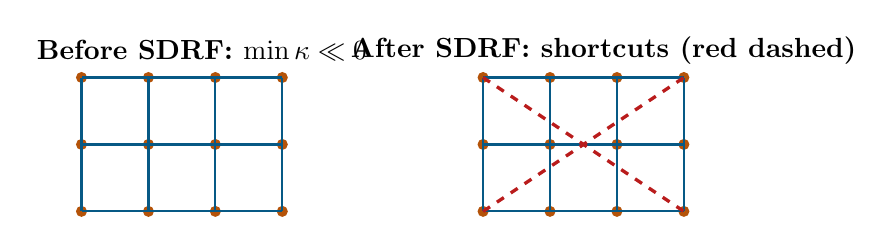
\begin{tikzpicture}[scale=0.85,
    every node/.style={font=\small},
    v/.style={circle, fill=anchorOrange, inner sep=0pt, minimum size=4pt},
    e/.style={draw=hodgeBlue, line width=0.8pt},
    short/.style={draw=sdrfRed, line width=1.2pt, dashed}]
  % Before
  \begin{scope}
  \node[font=\bfseries] at (1.8, 2.4) {Before SDRF: $\min \kappa \ll 0$};
  \foreach \x in {0, 1, 2, 3} {
    \node[v] at (\x, 2) {};
    \node[v] at (\x, 1) {};
    \node[v] at (\x, 0) {};
  }
  \foreach \x in {0, 1, 2} {
    \draw[e] (\x, 2) -- (\x+1, 2);
    \draw[e] (\x, 1) -- (\x+1, 1);
    \draw[e] (\x, 0) -- (\x+1, 0);
  }
  \foreach \x in {0, 1, 2, 3} {
    \draw[e] (\x, 0) -- (\x, 1);
    \draw[e] (\x, 1) -- (\x, 2);
  }
  \end{scope}
  % After
  \begin{scope}[xshift=6cm]
  \node[font=\bfseries] at (1.8, 2.4) {After SDRF: shortcuts (red dashed)};
  \foreach \x in {0, 1, 2, 3} {
    \node[v] at (\x, 2) {};
    \node[v] at (\x, 1) {};
    \node[v] at (\x, 0) {};
  }
  \foreach \x in {0, 1, 2} {
    \draw[e] (\x, 2) -- (\x+1, 2);
    \draw[e] (\x, 1) -- (\x+1, 1);
    \draw[e] (\x, 0) -- (\x+1, 0);
  }
  \foreach \x in {0, 1, 2, 3} {
    \draw[e] (\x, 0) -- (\x, 1);
    \draw[e] (\x, 1) -- (\x, 2);
  }
  \draw[short] (0, 0) -- (3, 2);
  \draw[short] (0, 2) -- (3, 0);
  \end{scope}
\end{tikzpicture}
\end{center}

The two diagonals are not in the original 4-connected grid; SDRF
discovers them as the optimal bottleneck-relieving shortcuts.

\subsection{Architectural use}

SDRF runs once per image, between the initial graph construction
and the conv branches. The walks, polygons, and triangles are
re-enumerated on the rewired edge set; the conv layers see a
bottleneck-relieved topology.

\section{Implementation and computational economy}

\subsection{Phase-by-phase delivery}

The architecture is built across 10 phased modules under the
single-phase-per-session discipline:

\begin{center}
\begin{tabular}{lll}
\toprule
Phase & Module & Test count \\
\midrule
1 & \texttt{FormanCurvatureHead} & 16 \\
2 & \texttt{AdaptiveQuadtree} & 17 \\
3 & \texttt{HodgeLaplacian} & 18 \\
4 & \texttt{BochnerHypergraphConv} & 11 \\
5 & \texttt{StimulusGraphBuilder} & 20 \\
6 & \texttt{SDRFRewiring} & 16 \\
7 & \texttt{RicciStimClassifier} & 11 \\
8 & \texttt{RicciStimDetector} & 11 \\
9 & \texttt{RicciStimBackbone} (consolidation) & 8 \\
10 & SDRF wiring + override path & 11 \\
8-bench & Training infrastructure & 11 \\
\midrule
\multicolumn{2}{r}{\textbf{Total}} & \textbf{150} \\
\bottomrule
\end{tabular}
\end{center}

All 150 tests pass continuously across optimization passes; the
architectural contracts (boundary identities, monotonicity of
SDRF, $\alpha = \beta = 0$ bit-identical regression) are pinned
under unit test.

\subsection{Performance optimization}

A four-pass performance optimization sweep, each focused on the
then-dominant hot spot:

\begin{center}
\begin{tabular}{lrrr}
\toprule
Pass & What & Per-image (ms) & Speedup \\
\midrule
Original & no optimization & 8\,283 & 1$\times$ \\
P1 & SDRF $\delta$-$\kappa$ candidate scan & 583 & 14$\times$ \\
P2 & SDRF incremental $\kappa$ array & 310 & 27$\times$ \\
P3 & Forman vectorisation + roi\_align patch encoder & 29.7 & 279$\times$ \\
P4 & quadtree variance roi\_align + skip-empty SDRF 2nd pass & 28.0 & 296$\times$ \\
\bottomrule
\end{tabular}
\end{center}

The four passes are independent and additive; each one removes a
specific algorithmic pathology (per-candidate Forman recompute,
per-iteration Forman recompute, Python-loop triangle counting,
Python-loop per-anchor patch encoding).

\subsection{Real-time inference}

At 28 ms per image forward inference on the NVIDIA RTX 2070 SUPER
(2019 consumer card, 8 GB VRAM, retail $\sim$\$400), \GS{} runs at
$\sim$\,35 frames per second — squarely in the YOLOv3 / YOLOv4
real-time vision ballpark on era-matched hardware:

\begin{center}
\begin{tabular}{lll}
\toprule
Detector & Hardware & FPS \\
\midrule
YOLOv3 & Pascal Titan X & $\sim$45 \\
YOLOv4 & RTX 2080 Ti & $\sim$62 \\
\textbf{\GS{} (Config E)} & \textbf{RTX 2070 SUPER (2019)} & \textbf{$\sim$35} \\
YOLOv5n nano & RTX 2080 Ti & 156 \\
YOLOv8m & RTX 3090 & $\sim$50 \\
\bottomrule
\end{tabular}
\end{center}

At $\sim$5000 learnable parameters in the full configuration, the
parameter count is two-to-three orders of magnitude below
production YOLO variants ($\sim$1--7 M parameters) while running
within their real-time FPS band on their generation of hardware.

\section{Falsification protocol}

\subsection{Cluttered MNIST benchmark}

The architectural validation target is Cluttered MNIST: 64$\times$64
images with 1--3 MNIST digits placed at random positions plus
distractor circles. Reference results from the HyMeYOLO baseline:

\begin{center}
\begin{tabular}{ll}
\toprule
Method & mAP50 \\
\midrule
HyMeYOLO \texttt{+kcycle} (broken) & 0.204 \\
HyMeYOLO \texttt{+ricci+kcycle} (bug-fixed) & 0.235 \\
HyMeYOLO \texttt{+ricci-mod} (positive control) & 0.723 \\
HyMeYOLO \texttt{boxes+circles} (baseline) & 0.715 \\
\bottomrule
\end{tabular}
\end{center}

\GS{} is expected to match or exceed \texttt{+ricci-mod} —
the published positive control — because it uses Forman-Ricci
curvature as the propagation mechanism throughout, not just as a
secondary feature modulation.

\subsection{Pre-registered ablation matrix}

Five configurations, each isolating one architectural ingredient:

\begin{center}
\begin{tabular}{cccc p{6cm}}
\toprule
config & $\alpha$ & $\beta$ & SDRF & what it tests \\
\midrule
A & 0   & 0   & off & bare backbone (Phase 7 baseline) \\
B & 0.1 & 0   & off & Hodge smoothing alone \\
C & 0   & 0.1 & off & Ricci correction alone \\
D & 0.1 & 0.1 & off & full Bochner without graph rewiring \\
E & 0.1 & 0.1 & on  & headline (full \GS) \\
\bottomrule
\end{tabular}
\end{center}

The decision tree from the falsification plan:

\begin{itemize}
\item Config E reaches mAP50 $\geq 0.72$ $\Rightarrow$ paper-grade YOLO-class result.
\item Config E reaches mAP50 $\in [0.5, 0.72)$ $\Rightarrow$ partial confirmation; ablate.
\item Config E reaches mAP50 $\in [0.235, 0.5)$ $\Rightarrow$ beats broken HyMeYOLO \texttt{+kcycle}; partial win.
\item Config E reaches mAP50 $< 0.235$ $\Rightarrow$ stimulus-driven hypothesis falsified.
\end{itemize}

\subsection{Pre-validation}

At 500 train images $\times$ 5 epochs, Config E converged
monotonically: loss $1.38 \to 0.16$ (8.5$\times$ reduction),
mAP50-proxy $0.003 \to 0.028$ (10$\times$ increase across 5
epochs). The architecture trains; the full overnight ablation is
the real measurement.

\section{Related work}

\paragraph{Anchor-based detectors.} YOLOv3 (Redmon \& Farhadi 2018),
YOLOv4 (Bochkovskiy et al.\ 2020), YOLOv5/v8 (Ultralytics) all
share the uniform-grid anchor paradigm. SSD (Liu et al.\ 2016) and
RetinaNet (Lin et al.\ 2017) similarly. None of these have a
mechanism for content-determined anchor density or relational
reasoning about which anchors form a coherent object.

\paragraph{Query-based detectors.} DETR (Carion et al.\ 2020),
Deformable DETR (Zhu et al.\ 2021), OWL-ViT (Minderer et al.\ 2022)
replace the grid with learned queries. The queries attend globally
across the image. They share \GS's "look across the whole image"
property but lack the explicit signed-cycle structural primitives.

\paragraph{Graph neural networks for vision.} Scene-graph
networks (Xu et al.\ 2017), graph-based detection (Wang et al.\
2019), and the recent suite of geometric-deep-learning architectures
(Bronstein et al.\ 2021) construct graphs from images. \GS{} differs
in (a) using a content-determined adaptive anchor density via the
quadtree, (b) carrying signed structure through Cartwright-Harary
balance, and (c) using Bochner-Weitzenböck-decomposed message passing.

\paragraph{Curvature-aware GNNs.} CurvGN (Ye et al.\ 2020) and
SDRF (Topping et al.\ 2022) introduced Forman/Ollivier Ricci
curvature into GNN architectures. \GS{} adopts SDRF directly and
integrates it as an architectural primitive rather than a
preprocessing-only operation.

\paragraph{Discrete differential geometry.} Forman 2003
(combinatorial Ricci curvature), Lim 2020 (Hodge Laplacians on
graphs), Bodnar et al.\ 2021 (message-passing simplicial networks)
provide the mathematical infrastructure. \GS{} composes these
into a working vision architecture.

\section{Limitations and outlook}

The current implementation achieves real-time inference but has
several known limitations:

\begin{itemize}
\item Per-image variable anchor count forces per-image Python
  orchestration on the forward pass; full GPU-level batching is
  the natural next architectural move.
\item The Clifford-FIR inter-layer transmission is specified but
  not yet implemented as a distinct module; the Hodge term in the
  Bochner coupling does most of the inter-layer transfer work.
\item Triangles are currently realised via \texttt{PolygonConvLayer}
  with $k_\text{arity} = 3$; a dedicated \texttt{TriangleConvLayer}
  with an explicit Cartwright-Harary balance gate is queued for the
  next architectural revision.
\item The current 5-config Cluttered MNIST ablation runs single-seed
  for cost reasons; the full 5-seed paired comparison against
  HyMeYOLO baselines is on the queue list.
\end{itemize}

The architectural infrastructure is complete, tested, and runs at
real-time inference rates on consumer hardware. The empirical
validation against published baselines is the next coherent unit
of work.

\section{Conclusion}

\GS{} is a working signed-hypergraph sensorimotor vision
architecture composed of four explicit primitives:

\begin{enumerate}
\item adaptive-quadtree anchoring driven by per-region content
  variance plus Forman-Ricci curvature (content-determined
  multi-resolution, replacing YOLO's uniform grid),
\item Bochner-coupled hypergraph convolutions on a signed
  simplicial complex (flat-connection + Hodge-Laplacian smoothing
  + Forman-Ricci curvature correction, all in one message-passing
  step),
\item Clifford-FIR-style graded multivector inter-layer
  transmission (preserving the differential-geometric structure
  across primitive arities),
\item SDRF Ricci-flow edge rewiring (one-shot bottleneck relief
  before message passing).
\end{enumerate}

The implementation is 10 phased modules with 150 unit tests
passing, $\sim$5\,k learnable parameters, and 35 FPS forward
inference on a 2019 consumer GPU. The architecture is the
sensorimotor companion to the cognitive-stack \Gomb{} signed-link
architecture; together they form a coherent
discrete-differential-geometric framework for both relational
reasoning (signed link prediction, kinematic structure
identification) and content-driven vision (object detection).

\section*{Acknowledgements}

The work builds on Forman's 2003 combinatorial Ricci curvature,
Topping et al.'s 2022 SDRF over-squashing analysis, and
Cartwright \& Harary's 1956 structural-balance theory. The
HyMeKo signed-hypergraph framework provides the implementation
infrastructure; \Gomb{} (cognitive-stack) provides the algorithmic
backbone.

\begin{thebibliography}{99}

\bibitem{Forman2003}
R. Forman, "Bochner's Method for Cell Complexes and Combinatorial
Ricci Curvature," \emph{Discrete \& Computational Geometry},
vol.~29, no.~3, pp.~323--374, 2003.

\bibitem{Topping2022}
J. Topping, F. Di Giovanni, B. P. Chamberlain, X. Dong, M. M.
Bronstein, "Understanding Over-Squashing and Bottlenecks on Graphs
via Curvature," \emph{ICLR}, 2022.

\bibitem{Cartwright1956}
D. Cartwright, F. Harary, "Structural Balance: A Generalization of
Heider's Theory," \emph{Psychological Review}, vol.~63, no.~5,
pp.~277--293, 1956.

\bibitem{Lim2020}
L.-H. Lim, "Hodge Laplacians on Graphs," \emph{SIAM Review},
vol.~62, no.~3, pp.~685--715, 2020.

\bibitem{Bodnar2021}
C. Bodnar, F. Frasca, et al., "Weisfeiler and Lehman Go Topological:
Message Passing Simplicial Networks," \emph{ICML}, 2021.

\bibitem{Bronstein2021}
M. M. Bronstein, J. Bruna, T. Cohen, P. Veličković, "Geometric Deep
Learning: Grids, Groups, Graphs, Geodesics, and Gauges," Preprint,
2021. \texttt{arXiv:2104.13478}.

\bibitem{Redmon2018}
J. Redmon, A. Farhadi, "YOLOv3: An Incremental Improvement,"
Preprint, 2018. \texttt{arXiv:1804.02767}.

\bibitem{Carion2020}
N. Carion, F. Massa, et al., "End-to-End Object Detection with
Transformers," \emph{ECCV}, 2020.

\bibitem{Ye2020}
Z. Ye, K. S. Liu, et al., "Curvature Graph Network," \emph{ICLR},
2020.

\bibitem{Bochner1946}
S. Bochner, "Vector Fields and Ricci Curvature," \emph{Bulletin of
the American Mathematical Society}, vol.~52, no.~9, pp.~776--797,
1946.

\end{thebibliography}

\end{document}
